%%%%%%%%%%%%%%%%%%%%%%%%%%%%%%%%%%%%%%%%%
% Arsclassica Article
% LaTeX Template
% Version 1.1 (1/8/17)
%
% This template has been downloaded from:
% http://www.LaTeXTemplates.com
%
% Original author:
% Lorenzo Pantieri (http://www.lorenzopantieri.net) with extensive modifications by:
% Vel (vel@latextemplates.com)
%
% License:
% CC BY-NC-SA 3.0 (http://creativecommons.org/licenses/by-nc-sa/3.0/)
%
%%%%%%%%%%%%%%%%%%%%%%%%%%%%%%%%%%%%%%%%%

%----------------------------------------------------------------------------------------
%	PACKAGES AND OTHER DOCUMENT CONFIGURATIONS
%----------------------------------------------------------------------------------------

\documentclass[
12pt, % Main document font size
a4paper, % Paper type, use 'letterpaper' for US Letter paper
oneside, % One page layout (no page indentation)
%twoside, % Two page layout (page indentation for binding and different headers)
headinclude,footinclude, % Extra spacing for the header and footer
BCOR5mm, % Binding correction
]{scrartcl}

\usepackage{amsmath}
%%%%%%%%%%%%%%%%%%%%%%%%%%%%%%%%%%%%%%%%%
% Arsclassica Article
% Structure Specification File
%
% This file has been downloaded from:
% http://www.LaTeXTemplates.com
%
% Original author:
% Lorenzo Pantieri (http://www.lorenzopantieri.net) with extensive modifications by:
% Vel (vel@latextemplates.com)
%
% License:
% CC BY-NC-SA 3.0 (http://creativecommons.org/licenses/by-nc-sa/3.0/)
%
%%%%%%%%%%%%%%%%%%%%%%%%%%%%%%%%%%%%%%%%%

%----------------------------------------------------------------------------------------
%	REQUIRED PACKAGES
%----------------------------------------------------------------------------------------

\usepackage[
nochapters, % Turn off chapters since this is an article        
beramono, % Use the Bera Mono font for monospaced text (\texttt)
eulermath,% Use the Euler font for mathematics
pdfspacing, % Makes use of pdftex’ letter spacing capabilities via the microtype package
dottedtoc % Dotted lines leading to the page numbers in the table of contents
]{classicthesis} % The layout is based on the Classic Thesis style

\usepackage{arsclassica} % Modifies the Classic Thesis package

\usepackage[T1]{fontenc} % Use 8-bit encoding that has 256 glyphs

\usepackage[utf8]{inputenc} % Required for including letters with accents

\usepackage{graphicx} % Required for including images
\graphicspath{{Figures/}} % Set the default folder for images

\usepackage{enumitem} % Required for manipulating the whitespace between and within lists

\usepackage{lipsum} % Used for inserting dummy 'Lorem ipsum' text into the template

\usepackage{subfig} % Required for creating figures with multiple parts (subfigures)

\usepackage{amsmath,amssymb,amsthm} % For including math equations, theorems, symbols, etc

\usepackage{varioref} % More descriptive referencing

%----------------------------------------------------------------------------------------
%	THEOREM STYLES
%---------------------------------------------------------------------------------------

\theoremstyle{definition} % Define theorem styles here based on the definition style (used for definitions and examples)
\newtheorem{definition}{Definition}

\theoremstyle{plain} % Define theorem styles here based on the plain style (used for theorems, lemmas, propositions)
\newtheorem{theorem}{Theorem}

\theoremstyle{remark} % Define theorem styles here based on the remark style (used for remarks and notes)

%----------------------------------------------------------------------------------------
%	HYPERLINKS
%---------------------------------------------------------------------------------------

\hypersetup{
%draft, % Uncomment to remove all links (useful for printing in black and white)
colorlinks=true, breaklinks=true, bookmarks=true,bookmarksnumbered,
urlcolor=webbrown, linkcolor=RoyalBlue, citecolor=webgreen, % Link colors
pdftitle={}, % PDF title
pdfauthor={\textcopyright}, % PDF Author
pdfsubject={}, % PDF Subject
pdfkeywords={}, % PDF Keywords
pdfcreator={pdfLaTeX}, % PDF Creator
pdfproducer={LaTeX with hyperref and ClassicThesis} % PDF producer
} % Include the structure.tex file which specified the document structure and layout

\hyphenation{Fortran hy-phen-ation} % Specify custom hyphenation points in words with dashes where you would like hyphenation to occur, or alternatively, don't put any dashes in a word to stop hyphenation altogether

%----------------------------------------------------------------------------------------
%	TITLE AND AUTHOR(S)
%----------------------------------------------------------------------------------------

\title{\normalfont\spacedallcaps{MMI Display Interface Panel}} % The article title

\subtitle{11-01-001-6} % Uncomment to display a subtitle

%\author{\spacedlowsmallcaps{John Smith* \& James Smith\textsuperscript{1}}} % The article author(s) - author affiliations need to be specified in the AUTHOR AFFILIATIONS block

\date{} % An optional date to appear under the author(s)

%----------------------------------------------------------------------------------------

\begin{document}

%----------------------------------------------------------------------------------------
%	HEADERS
%----------------------------------------------------------------------------------------

\renewcommand{\sectionmark}[1]{\markright{\spacedlowsmallcaps{#1}}} % The header for all pages (oneside) or for even pages (twoside)
%\renewcommand{\subsectionmark}[1]{\markright{\thesubsection~#1}} % Uncomment when using the twoside option - this modifies the header on odd pages
\lehead{\mbox{\llap{\small\thepage\kern1em\color{halfgray} \vline}\color{halfgray}\hspace{0.5em}\rightmark\hfil}} % The header style

\pagestyle{scrheadings} % Enable the headers specified in this block

%----------------------------------------------------------------------------------------
%	TABLE OF CONTENTS & LISTS OF FIGURES AND TABLES
%----------------------------------------------------------------------------------------

\maketitle % Print the title/author/date block

\setcounter{tocdepth}{5} % Set the depth of the table of contents to show sections and subsections only

\tableofcontents % Print the table of contents

%\listoffigures % Print the list of figures

%\listoftables % Print the list of tables

%----------------------------------------------------------------------------------------
%	ABSTRACT
%----------------------------------------------------------------------------------------

%\newpage
\section*{Abstract} % This section will not appear in the table of contents due to the star (\section*)

%\lipsum[1] % Dummy text

This module consists of an TFT touchscreen shield mounted on Arduino Uno. This is used to display the name and manufacturer of any product.
%----------------------------------------------------------------------------------------
%	AUTHOR AFFILIATIONS
%----------------------------------------------------------------------------------------

%\let\thefootnote\relax\footnotetext{* \textit{Department of Biology, University of Examples, London, United Kingdom}}

%\let\thefootnote\relax\footnotetext{\textsuperscript{1} \textit{Department of Chemistry, University of Examples, London, United Kingdom}}

%----------------------------------------------------------------------------------------

\newpage % Start the article content on the second page, remove this if you have a longer abstract that goes onto the second page

\section{Components}

\begin{enumerate}
\item $2.4"$ TFT Touch Shield for Arduino
\item Arduino Uno
\item USB Type A (male) to Type B (male) cable
\item $5.0V$, $1A$ power supply with USB Type A (female) connector
\item micro-SD card (less than or equal to $4GB$)
\end{enumerate}
%----------------------------------------------------------------------------------------
%	INTRODUCTION
%----------------------------------------------------------------------------------------

\section{System Level Block Diagram}

\begin{figure}[tbh]
\centering
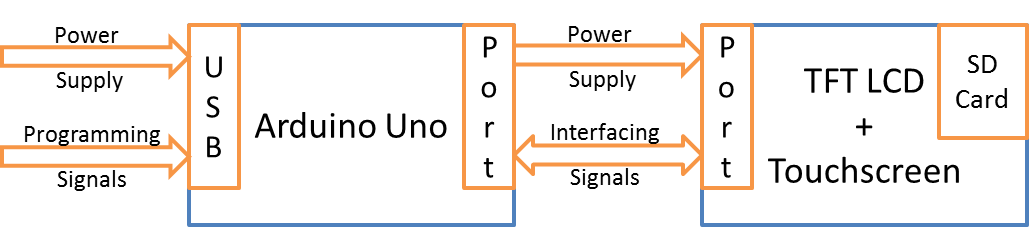
\includegraphics[width=1\columnwidth]{Block_diag.png} 
\caption{System level block diagram} % The text in the square bracket is the caption for the list of figures while the text in the curly brackets is the figure caption
\label{fig:block_diag}
\end{figure}
 
%----------------------------------------------------------------------------------------
%	INTRODUCTION
%----------------------------------------------------------------------------------------

\section{Hardware Setup}

\subsection{for usage}

\begin{
Make sure TFT Touch Shield is mounted on arduino uno and micro-SD card is inserted in the slot at the bottom of the TFT Touch Shield.

As shown in figure \ref{fig:block_diag} the TFT Touch Shield is plugged onto Arduino Uno ports for interfacing. Vdd and Gnd pins on both
boards should be matched for proper mounting.
\textit{If you are setting up arduino uno first time on this computer, do not mount TFT touchsreen shield on the arduino board yet. It will be mounted
after arduino uno setup section.}\\

\subsection{for programming}
The USB cable's Type B end is connected to the Arduino Uno board and this cable provides both the power and programming signals.
In case one wants to program the module, USB Type A end or cable should be connected to a computer else it should be connected to
a $5V$, $1A$ power supply. In both cases Arduino and LCD screen should power up and you should be able to see red lights on Arduino board
and backlight or any random display on LCD.\\
 

%----------------------------------------------------------------------------------------
%	METHODS
%----------------------------------------------------------------------------------------

\section{Programming Instructions}

\subsection{Arduino Uno Setup}

%\lipsum[5] % Dummy text
If the module is connected to computer for programming, following instructions need to be followed

\paragraph{Installing software}
The Arduino Uno is programmed using the Arduino Software (IDE), Arduino's Integrated Development Environment.
Double click on \textit{arduino-1.8.5-windows.exe} and please allow the driver installation process when you get 
a warning from the operating system.\\

\begin{figure}[tbh]
%\centering
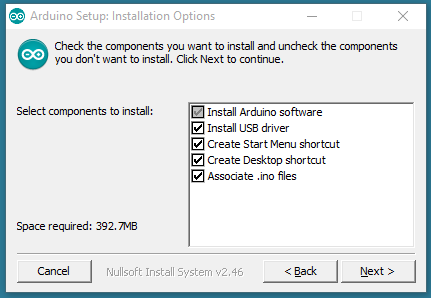
\includegraphics[width=0.75\columnwidth]{DRV_Capture1.png} 
%\caption{System level block diagram} % The text in the square bracket is the caption for the list of figures while the text in the curly brackets is the figure caption
\end{figure}

\flushleft Choose the components to install

\begin{figure}[tbh]
%\centering
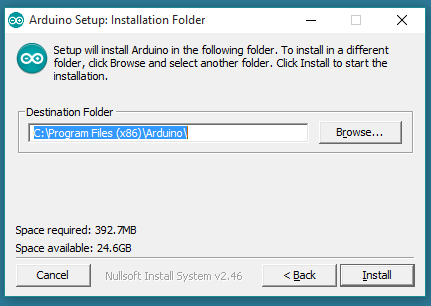
\includegraphics[width=0.75\columnwidth]{DRV_Capture2.png} 
%\caption{System level block diagram} % The text in the square bracket is the caption for the list of figures while the text in the curly brackets is the figure caption
\end{figure}

\flushleft Choose the installation directory (we suggest to keep the default one)

\begin{figure}[tbh]
%\centering
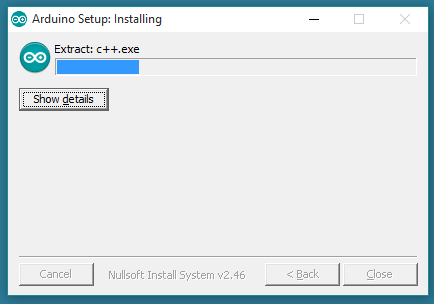
\includegraphics[width=0.75\columnwidth]{DRV_Capture3.png} 
%\caption{System level block diagram} % The text in the square bracket is the caption for the list of figures while the text in the curly brackets is the figure caption
\end{figure}

\newpage
\flushleft The process will extract and install all the required files to execute properly the Arduino Software (IDE)\\


\paragraph{Installing additional libraries}
Unzip libraries.rar and copy the folders $\mathit{SPFD5408-master}$ etc to $\mathit{C:\textbackslash Program Files (x86)\textbackslash Arduino\textbackslash libraries}$

%\paragraph{Installing additional libraries}

%------------------------------------------------

\paragraph{Connecting board}

Connect your Uno board with an A B USB cable; sometimes this cable is called a USB printer cable
\begin{figure}[tbh]
%\centering
\subfloat{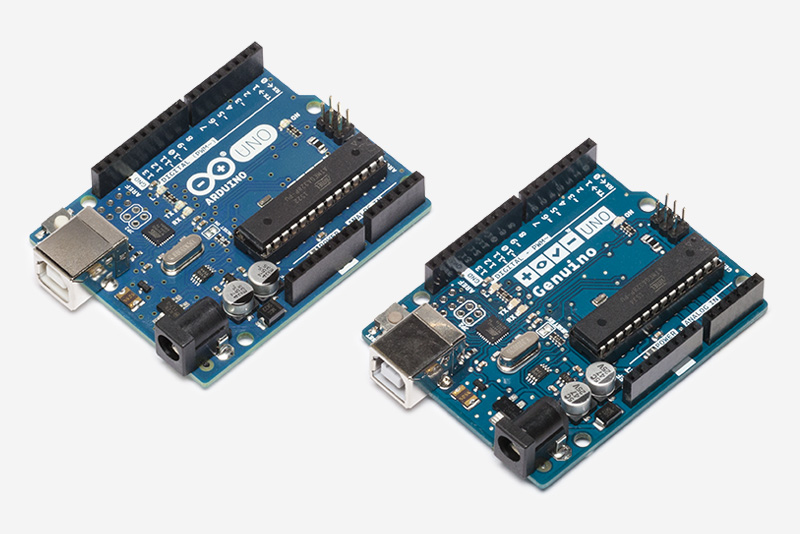
\includegraphics[width=.50\columnwidth]{A000066_iso_both.jpg}} \quad
\subfloat{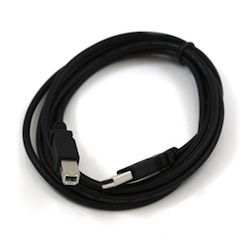
\includegraphics[width=.30\columnwidth]{USBCable.jpg}} \\
%\caption{System level block diagram} % The text in the square bracket is the caption for the list of figures while the text in the curly brackets is the figure caption
\end{figure}


The USB connection with the PC is necessary to program the board and not just to power it up. The Uno automatically draw power from either the USB or an external power supply. Connect the board to your computer using the USB cable. The green power LED (labelled PWR) should go on.


\paragraph{Install the board drivers}

If you downloaded and expanded the Zip package or, for some reason, the board wasn't properly recognized, please follow the procedure below.

\begin{itemize}[leftmargin=*]
\item Click on the Start Menu, and open up the Control Panel.
\item While in the Control Panel, navigate to System and Security. Next, click on System. Once the System window is up, open the Device Manager.
\item Look under Ports (COM \& LPT). You should see an open port named "Arduino UNO (COMxx)". If there is no COM \& LPT section, look under 
"Other Devices" for "Unknown Device".
\item Right click on the "Arduino UNO (COmxx)" port and choose the "Update Driver Software" option.
\item Next, choose the "Browse my computer for Driver software" option.
\item Finally, navigate to and select the driver file named "arduino.inf", located in the "Drivers" folder of the Arduino Software download 
(not the "FTDI USB Drivers" sub-directory). If you are using an old version of the IDE (1.0.3 or older), choose the Uno driver file named "Arduino UNO.inf"
\item Windows will finish up the driver installation from there.
\end{itemize}


\paragraph{Open your first sketch}

Open the LED blink example sketch: $File > Examples >01.Basics > Blink$.

\begin{figure}[tbh]
%\centering
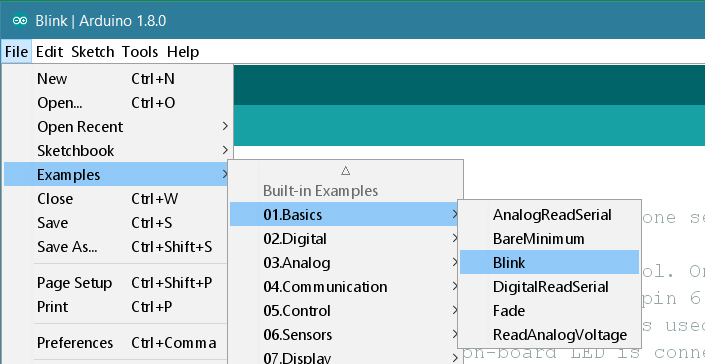
\includegraphics[width=0.9\columnwidth]{UNO_Load_Blink.jpg} 
%\caption{System level block diagram} % The text in the square bracket is the caption for the list of figures while the text in the curly brackets is the figure caption
\end{figure}

\paragraph{Select your board type and port}
You'll need to select the entry in the $Tools > Board$ menu that corresponds to your Arduino or Genuino board.

\begin{figure}[tbh]
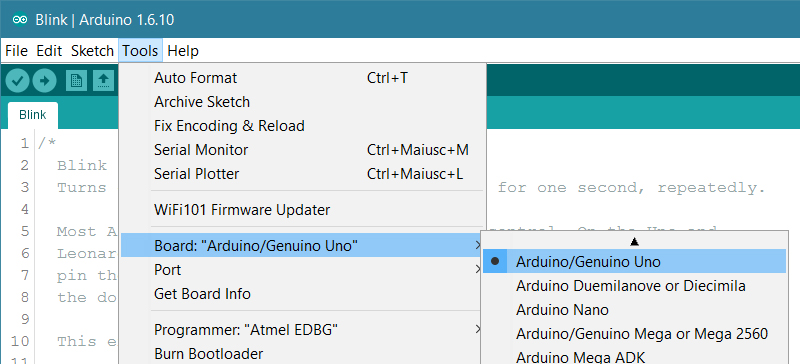
\includegraphics[width=0.9\columnwidth]{UNO_BoardType.jpg} 
\end{figure}

\newpage
Select the serial device of the board from the Tools | Serial Port menu. This is likely to be COM3 or higher (COM1 and COM2 are usually reserved for hardware serial ports). To find out, you can disconnect your board and re-open the menu; the entry that disappears should be the Arduino or Genuino board. Reconnect the board and select that serial port.

\begin{figure}[tbh]
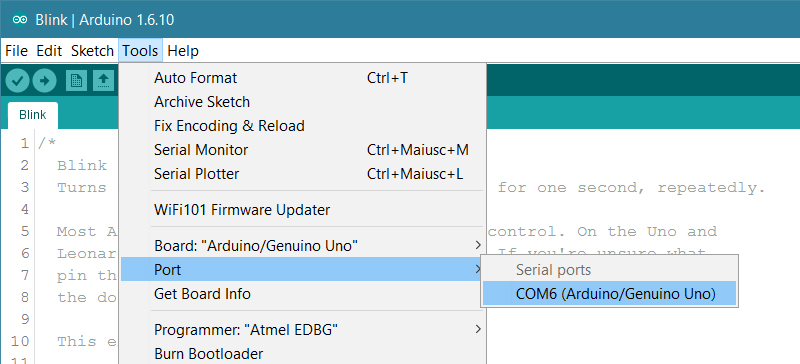
\includegraphics[width=0.9\columnwidth]{UNO_Port.jpg} 
\end{figure}


\paragraph{Upload the program}
Now, simply click the "Upload" button in the environment. Wait a few seconds - you should see the RX and TX leds on the board flashing. If the upload is successful, the message "Done uploading." will appear in the status bar.

\begin{figure}[tbh]
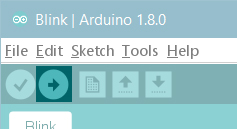
\includegraphics[width=0.5\columnwidth]{UNO_Upload.png} 
\end{figure}

A few seconds after the upload finishes, you should see the pin 13 (L) LED on the board start to blink (in orange). If it does, congratulations! You've gotten Arduino or Genuino up-and-running. If you have problems, please see the \href{https://www.arduino.cc/en/Guide/Troubleshooting}{troubleshooting suggestions}.






\subsection{Upload our program}

\begin{itemize}
\item Open \textit{tftpaint.ino} in Arduino by double clicking the file
\item Click the upload button (looks like \textit{forward arrow} symbol)
\end{itemize}


\subsection{Upload bmp in memory card}
\begin{itemize}
\item Copy files \textit{screen.bmp, screen2.bmp, screen3.bmp} to the memory card (less than or equal to 4 GB)
\item Insert the memory card to slot in LCD
\end{itemize}
%------------------------------------------------

%----------------------------------------------------------------------------------------
%	RESULTS AND DISCUSSION
%----------------------------------------------------------------------------------------

\section{Setup Required}

Reference to Figure~\vref{fig:gallery}. % The \vref command specifies the location of the reference

\begin{figure}[tb]
\centering 
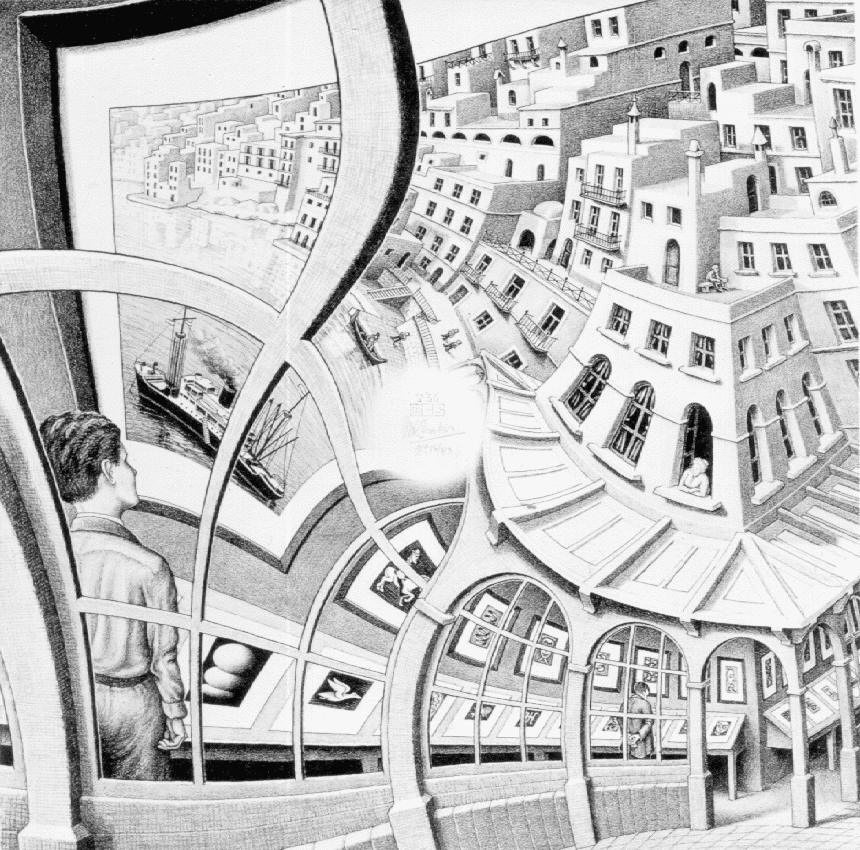
\includegraphics[width=0.5\columnwidth]{GalleriaStampe} 
\caption[An example of a floating figure]{An example of a floating figure (a reproduction from the \emph{Gallery of prints}, M.~Escher,\index{Escher, M.~C.} from \url{http://www.mcescher.com/}).} % The text in the square bracket is the caption for the list of figures while the text in the curly brackets is the figure caption
\label{fig:gallery} 
\end{figure}

\lipsum[10] % Dummy text

%------------------------------------------------

\subsection{Subsection}

\lipsum[11] % Dummy text

\subsubsection{Subsubsection}

\lipsum[12] % Dummy text

\begin{description}
\item[Word] Definition
\item[Concept] Explanation
\item[Idea] Text
\end{description}

\lipsum[12] % Dummy text

\begin{itemize}[noitemsep] % [noitemsep] removes whitespace between the items for a compact look
\item First item in a list
\item Second item in a list
\item Third item in a list
\end{itemize}

\subsubsection{Table}

\lipsum[13] % Dummy text

\begin{table}[hbt]
\caption{Table of Grades}
\centering
\begin{tabular}{llr}
\toprule
\multicolumn{2}{c}{Name} \\
\cmidrule(r){1-2}
First name & Last Name & Grade \\
\midrule
John & Doe & $7.5$ \\
Richard & Miles & $2$ \\
\bottomrule
\end{tabular}
\label{tab:label}
\end{table}

Reference to Table~\vref{tab:label}. % The \vref command specifies the location of the reference

%------------------------------------------------

\subsection{Figure Composed of Subfigures}

Reference the figure composed of multiple subfigures as Figure~\vref{fig:esempio}. Reference one of the subfigures as Figure~\vref{fig:ipsum}. % The \vref command specifies the location of the reference

\lipsum[15-18] % Dummy text

\begin{figure}[tb]
\centering
\subfloat[A city market.]{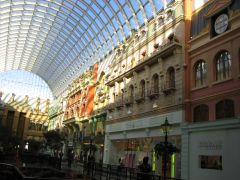
\includegraphics[width=.45\columnwidth]{Lorem}} \quad
\subfloat[Forest landscape.]{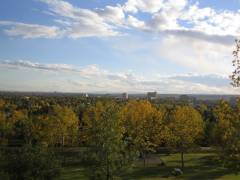
\includegraphics[width=.45\columnwidth]{Ipsum}\label{fig:ipsum}} \\
\subfloat[Mountain landscape.]{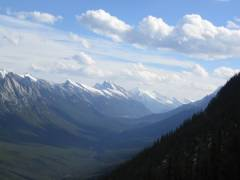
\includegraphics[width=.45\columnwidth]{Dolor}} \quad
\subfloat[A tile decoration.]{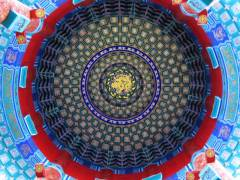
\includegraphics[width=.45\columnwidth]{Sit}}
\caption[A number of pictures.]{A number of pictures with no common theme.} % The text in the square bracket is the caption for the list of figures while the text in the curly brackets is the figure caption
\label{fig:esempio}
\end{figure}

%----------------------------------------------------------------------------------------
%	INTRODUCTION
%----------------------------------------------------------------------------------------

\section{Setup files (Software)}

A statement requiring citation \cite{Figueredo:2009dg}.

\lipsum[1-3] % Dummy text

Some mathematics in the text: $\cos\pi=-1$ and $\alpha$.

%----------------------------------------------------------------------------------------
%	BIBLIOGRAPHY
%----------------------------------------------------------------------------------------

\renewcommand{\refname}{\spacedlowsmallcaps{References}} % For modifying the bibliography heading

\bibliographystyle{unsrt}

\bibliography{sample} % The file containing the bibliography

%----------------------------------------------------------------------------------------

\end{document}